%ch.tex


\chapter{The domain model as abstract syntax}
\begin{center}
{\small\em In which Pooh and Piglet understand the value of pipelines}
\end{center}

\begin{figure}[tbp]
\begin{center}
{ 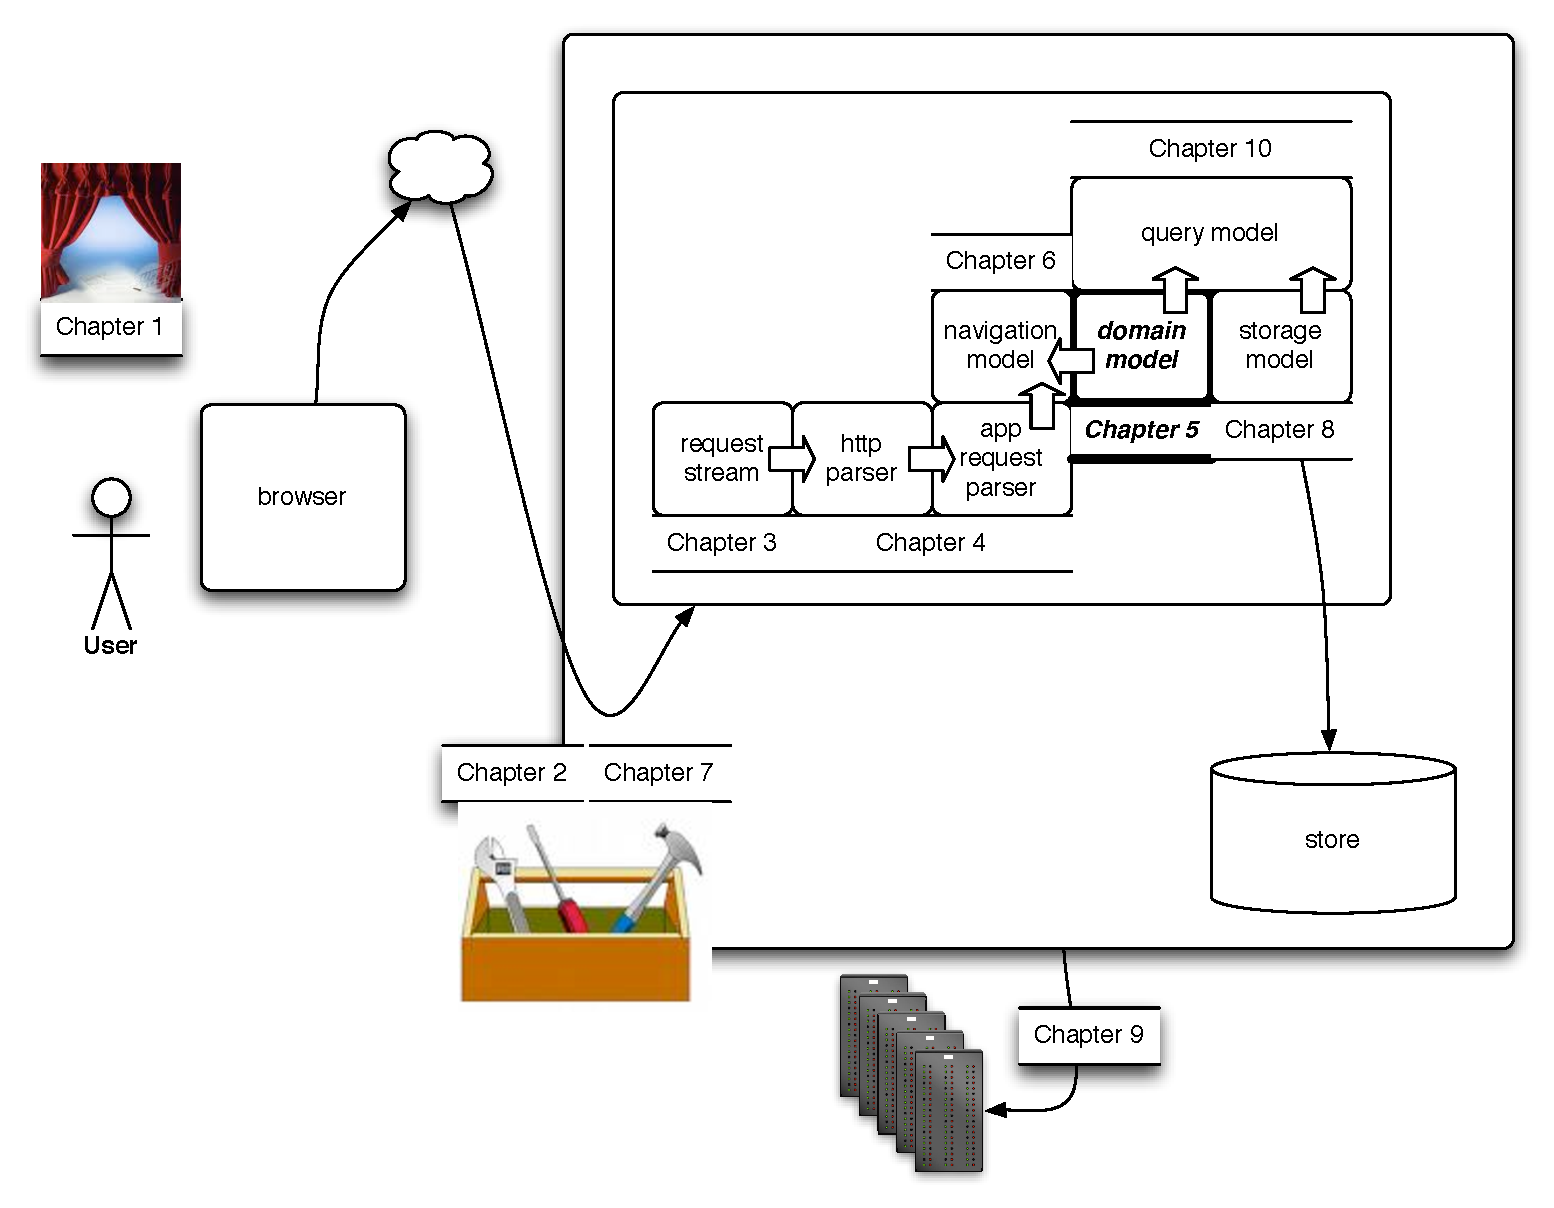
\includegraphics[scale=.35]{/Users/lgm/work/src/projex/biosimilarity/trace/src/main/book/content/figures/MonadicDesignPatternsChapterMapFocus5.pdf} }
\caption{ Chapter map }
\end{center}
\end{figure}

TBD
\section{Our abstract syntax}

\paragraph{Abstract syntax}
%For our example we'll need a toy language.
Fittingly for a book about \texttt{Scala} we'll use the
$\lambda$-calculus as our toy language. \footnote{A word to the wise:
  even if you are an old hand at programming language semantics, even
  if you know the $\lambda$-calculus like the back of your hand, you
  are likely to be surprised by some of the things you see in the next
  few sections. Just to make sure that everyone gets a chance to look
  at the formalism as if it were brand new, a few recent theoretical
  developments have been thrown in. So, watch out!} The core
\textit{abstract} syntax of the lambda calculus is given by the
following \textit{EBNF} grammar.

\begin{mathpar}
  \inferrule* [lab=expression] {} {{M,N} ::=}
  \and
  \inferrule* [lab=mention] {} {x}
  \and
  \inferrule* [lab=abstraction] {} {\;| \; \lambda x . M}
  \and
  \inferrule* [lab=application] {} {\;| \; M N}
\end{mathpar} 

Informally, this is really a language of pure variable management. For
example, if the expression $M$ mentions $x$, then $\lambda x. M$ turns
$x$ into a variable in $M$ and provides a means to substitute values
into $M$, via application. Thus, $(\lambda x.M)N$ will result in a new
term, sometimes written $M[N/x]$, in which every occurrence of $x$ has
been replaced by an occurrence of $N$. Thus, $(\lambda x.x)M$ yields
$M$, illustrating the implementation in the $\lambda$-calculus of the
identity function. It turns out to be quite remarkable what you can do
with pure variable management.


\section{Our application domain model}

TBD
\section{A transform pipeline}

TBD

% \section{Existence problems}
% We begin with some metamathematics.
% All problems about the existence of maps can be cast into one of the
% following two forms, which are in a sense mutually dual.

% \noindent
% {\bf The Extension Problem}\index{extension problem} \    %%% NB index entry tag
% Given an inclusion $ A \stackrel{i}{\hookrightarrow} X $, and a map
% $ A \stackrel{f}{\rightarrow} Y $,
% does there exist a map $f^{\dagger}:X\to Y$ such that
% $f^{\dagger}$ agrees with $f$ on $A$?

% Here the appropriate source category for maps should be clear from the
% context and, moreover, commutativity through a
% candidate $f^{\dagger}$ is precisely
% the restriction requirement; that is,
% $$f^{\dagger}   :  f^{\dagger}\circ i = f^{\dagger}|_A = f\,. $$
% If such an $f^{\dagger}$ exists\footnote{${}^{\dagger}$ suggests striving
% for perfection, crusading}, then it is called an {\bf
% extension}\index{extension!of a map|bi} of $f$ and is said to {\bf
% extend}\index{extend|bi} $f$. In any diagrams, the presence of
% a dotted arrow or an arrow carrying a ? indicates a pious hope, in no way
% begging the question of its existence. Note that we shall usually
% omit $\circ$ from composite maps.

% \noindent
% {\bf The Lifting Problem}\index{lifting problem} \
% Given a pair of maps $E \stackrel{p}{\rightarrow}B$ and $X \stackrel{f}
% {\rightarrow} B $,
% does there exist a map $f^{\circ} : X \to E$, with
% $pf^{\circ} = f  $?


% That {\em all\/} existence problems about maps are essentially of one
% type or
% the other from these two is seen as follows. Evidently, all existence problems
% are representable by triangular diagrams\index{triangular diagrams} and it
% is easily seen that there are only these six possibilities:
% \begin{center}\begin{picture}(300,70)  %augch2 75
% \put(5,60){\vector(1,0){30}}
% \put(55,60){\vector(1,0){30}}
% \put(135,60){\vector(-1,0){30}}
% \put(185,60){\vector(-1,0){30}}
% \put(235,60){\vector(-1,0){30}}
% \put(285,60){\vector(-1,0){30}}
% \put(0,55){\vector(0,-1){30}}
% \put(50,55){\vector(0,-1){30}}
% \put(100,25){\vector(0,1){30}}
% \put(150,25){\vector(0,1){30}}
% \put(200,55){\vector(0,-1){30}}
% \put(250,55){\vector(0,-1){30}}
% \put(28,33){\small ?}
% \put(78,33){\small ?}
% \put(128,33){\small ?}
% \put(178,33){\small ?}
% \put(228,33){\small ?}
% \put(278,33){\small ?}
% \put(10,3){\bf 1}
% \put(60,3){\bf 2}
% \put(110,3){\bf 3}
% \put(160,3){\bf 4}
% \put(210,3){\bf 5}
% \put(260,3){\bf 6}
% \put(35,55){\vector(-1,-1){30}}
% \put(155,25){\vector(1,1){30}}
% \put(135,55){\vector(-1,-1){30}}
% \put(55,25){\vector(1,1){30}}
% \put(235,55){\vector(-1,-1){30}}
% \put(255,25){\vector(1,1){30}}
% \end{picture}\end{center}



% \begin{figure}
% \begin{picture}(300,220)(0,0)
% \put(-20,-20){\resizebox{20 cm}{!}{\includegraphics{3dpdf}}}
% \put(260,-10){\resizebox{15 cm}{!}{\includegraphics{contpdf}}}
% \put(220,80){$\beta$}
% \put(400,-10){$N$}
% \put(260,170){$\beta$}
% \put(90,15){$N$}
% \end{picture}
% \caption{{\em The log-gamma family of densities with central mean
% $<N> \, = \frac{1}{2}$ as a surface and as a contour plot. }}
% \label{pdf}
% \end{figure}

\newpage
